\documentclass[12pt,a4paper,titlepage,twoside]{article}
\usepackage[T1]{fontenc}
\usepackage[cp1250]{inputenc}
\usepackage[english,polish]{babel}
\usepackage[T1]{polski}
\usepackage{times}
\usepackage{fancyhdr}
\usepackage{hyperref}
\usepackage{graphicx}
\usepackage{slashbox}
\usepackage{sistyle}
\usepackage{amsfonts}
\usepackage{latexsym}
%\usepackage{notebook2e, latexsym}

\hypersetup
{
	bookmarksnumbered=true,
	colorlinks=true,
	linkcolor=blue,
	bookmarksopen=true,
	bookmarksopenlevel=2,
	pdfstartview={FitH}
}

\SIdecimalsign{,}

\setlength{\textheight}{24cm}
\setlength{\textwidth}{16cm}
\setlength{\footskip}{10mm}
\setlength{\oddsidemargin}{0mm}
\setlength{\evensidemargin}{0mm}
\setlength{\topmargin}{0mm}
\setlength{\headsep}{5mm}
\setlength{\headheight}{15.0pt}

\pagestyle{fancy}
\fancyhead{}
\fancyhead[LE,RO]{\textsf{\thepage}}
\fancyhead[RE,LO]{\textsf{Szeregowanie zada� jednorodnych}}
\fancyhead[CE,CO]{\ }
\fancyfoot[LE,RO]{\ }
\fancyfoot[RE,LO]{\ }
\fancyfoot[CE,CO]{\ }
\renewcommand{\headrulewidth}{0.4pt}
\renewcommand{\footrulewidth}{0.4pt}

\begin{titlepage}
\title{Przetwarzanie r�wnoleg�e \\ Szeregowanie zada� jednorodnych}
\author{Bartosz Kukawka (75911) \\ Marcin Miko�ajczak (75922) \\ Grupa I3A}
\end{titlepage}

\begin{document}

\maketitle
\tableofcontents

\newpage

\section{Sformu�owanie problemu}
Przedmiotem niniejszego sprawozdania jest analiza problemu przetwarzania r�wnoleg�ego w o�mioprocesorowym systemie przetwarzania o topologii sze�cianu, kt�ry cechuje mo�liwo�� jednoczesnego wykonywania oblicze� i~przesy�ania danych przez ka�dy z~jego procesor�w. Dodatkowo zak�ada si�, �e w~chwili zerowej oblicze� wszystkie dane potrzebne do ich wykonania znajduj� si� w~jednym z~naro�nik�w wspomnianego sze�cianu.

Analizowany system wraz z~przyj�tymi oznaczeniami procesor�w przedstawiaj� pogl�dowo rysunki \ref{fig:cube} i~\ref{fig:flat}. Procesor, kt�ry pocz�tkowo dysponuje wszystkimi danymi, zosta� oznaczony numerem 0. Dalsza numeracja wynika z~odleg�o�ci od �r�d�a danych. Po�r�d procesor�w o r�wnej odleg�o�ci numeracja zosta�a przydzielona na podstawie rzutu z~rysunku \ref{fig:cube} w~kolejno�ci zgodnej z~ruchem wskaz�wek zegara, poczynaj�c od procesor�w na g�rnej, tylnej kraw�dzi sze�cianu. Inny widok omawianego systemu przedstawia rysunek \ref{fig:flat}.

\begin{figure}[h!]
\centering
\includegraphics[trim=0 15mm 0 15mm, clip]{cube}
\caption{Schemat analizowanego systemu przetwarzania}
\label{fig:cube}
\end{figure}

\begin{figure}[p]
\centering
\includegraphics[trim=0 0 0 0, clip]{flat}
\caption{Schemat analizowanego systemu przetwarzania c.d.}
\label{fig:flat}
\end{figure}

\section{Model w~�rodowisku Parastation}
Opisany wy�ej system przetwarzania zosta� zamodelowany w~�rodowisku Parastation w~spos�b przedstawiony na rysunku \ref{fig:parastation}. Niewykorzystywane procesory nie otrzyma�y numeracji, a~niewykorzystywane ��cza nie zosta�y uwzgl�dnione na rysunku.

\begin{figure}[p]
\centering
\includegraphics[trim=0 0 0 0, clip]{parastation}
\caption{Model systemu w~�rodowisku Parastation}
\label{fig:parastation}
\end{figure}

\section{Analiza problemu}
Celem analizy by�o znalezienie odpowiedzi na pytanie o optymalny dla rozwa�anego systemu przetwarzania plan przesy�ania danych i wykonywania oblicze�. Plan ten powinien uwzgl�dnia� podzia� transmisji na odpowiedni� ilo�� faz oraz ilo�ci danych przesy�anych w~ich trakcie, d���c do jak najwcze�niejszego (a~wi�c jednoczesnego) zako�czenia oblicze� na wszystkich procesorach.

Odpowiedzi na postawione wy�ej pytanie udzieli�o rozwi�zanie odpowiedniego problemu programowania liniowego, kt�ry zosta� sformu�owany w~spos�b opisany w~kolejnych podpunktach.

\subsection{Idea rozwi�zania}
Ze wzgl�du na mo�liwo�� otrzymywania danych z wielu �r�de�, jako podstaw� w sformu�owaniu odpowiedniego problemu programowania liniowego przyj�to podej�cie nazwane przez autor�w niniejszego sprawozdania "systemem kana��w". W r�wnaniach opisanych w kolejnych podpunktach pos�u�ono si� 16 kana�ami przesy�ania danych ($i = 0 \ldots 15$), odpowiadaj�cymi r�nym �cie�kom, kt�rymi dane mog� dociera� do procesor�w ($j = 0 \ldots 7$). Dla procesor�w warstwy 1 (procesory 1, 2, 3) jest tylko 1 taka �cie�ka, dla warstwy 2 (procesory 4, 5, 6) - 2 �cie�ki, a dla warstwy 3 (procesor 7) - 6 �cie�ek. W celu usprawnienia procesu oblicze�, dane przesy�ane s� ka�dym kana�em w $m$ pakietach, odpowiadaj�cym $m$ fazom oblicze� ($k = m-1 \ldots 0$). Po skompletowaniu pakiet�w ze wszystkich docieraj�cych do procesora kana��w dla danej fazy nast�puje r�wnoleg�� przeliczenie cz�ci otrzymanych danych oraz przes�anie reszty do kolejnych procesor�w, je�li takie istniej�. Proces powtarza si� $m$ razy, do chwili zako�czenia przetwarzania wszystkich danych.\\*

Podsumowuj�c powy�szy opis, mo�na wyr�ni� nast�puj�ce kluczowe poj�cia, kt�re b�d� wykorzystywane w dalszym ci�gu sprawozdania:
\begin{description}
\item[kana� $i$] -- �cie�ka, kt�r� dane docieraj� do procesora $j$ docelowego dla tego kana�u; kana�em wysy�ane s� pakiety $(i,k: k = m-1 \ldots 0)$
\item[pakiet $(i,k)$] -- pojedy�cza transmisja danych pomi�dzy procesorami, s� to dane przesy�ane do procesora docelowego dla kana�u $i$ w fazie $k$; pakiet zawiera paczk� $(i,k)$ oraz paczki $(p: p \in after(i), k)$
\item[paczka $(i,k)$] -- fragment pakietu zawieraj�cy dane do przetworzenia  lokalnego w fazie $k$ na procesorze docelowym kana�u $i$ 
\end{description}

Przedstawione wy�ej poj�cia obrazuje fragment diagramu Gantta dla wybranego procesora przedstawiony na rysunku \ref{fig:example}.

\begin{figure}[h]
\centering
\includegraphics[width=\textwidth, trim=0 0 0 0, clip]{example}
\caption{Fragment diagramu Gantta obrazuj�cy wykorzystywane w sprawozdaniu poj�cia}
\label{fig:example}
\end{figure}

\newpage

\subsection{Funkcje opisuj�ce system kana��w}
\begin{description}
\item[$channels(j)$] -- zbi�r numer�w kana��w ko�cz�cych si� w procesorze $j$
\item[$before(i)$] -- zbi�r numer�w kana��w, od kt�rych zale�y kana� $i$, tzn. takich, kt�rymi przesy�anie w danej fazie musi si� zako�czy� przed wys�aniem pakietu kana�em $i$
\item[$after(i)$] -- zbi�r numer�w kana��w, kt�re zale�� od kana�u $i$, tzn. takich, kt�rymi nie mo�na wys�a� w danej fazie pakiet�w, dop�ki nie zostanie zako�czona transmisja kana�em $i$
\end{description}

Warto�ci wymienionych wy�ej funkcji wynikaj� bezpo�rednio ze struktury rozwa�anego systemu przetwarzania. Przedstawiaj� je tabele \ref{tab:channels}, \ref{tab:before} i \ref{tab:after}.

\begin{table}[p]
\centering
\begin{tabular}{|r|c|c|c|c|c|c|c|c|}
\hline
$j$ & $0$ & $1$ & $2$ & $3$ & $4$ & $5$ & $6$ & $7$ \\
\hline
$channels(j)$ & ${}$ & ${1}$ & ${2}$ & ${3}$ & ${4,6}$ & ${7,8}$ & ${5,9}$ & ${10,11,12,13,14,15}$ \\
\hline
\end{tabular}
\caption{channels}
\label{tab:channels}
\end{table}

\begin{table}[p]
\centering
\begin{tabular}{|r|c|c|c|c|c|c|c|c|c|c|c|c|c|c|c|c|}
\hline
$i$ &  $0$ &  $1$ &  $2$ &  $3$
    &  $4$ &  $5$ &  $6$ &  $7$
    &  $8$ &  $9$ & $10$ & $11$
    & $12$ & $13$ & $14$ & $15$ \\
\hline
$before(i)$ &    ${0}$ &  ${0}$ &    ${0}$ &    ${0}$ 
            &    ${1}$ &  ${1}$ &    ${2}$ &    ${2}$
            &    ${3}$ &  ${3}$ &    ${4}$ &    ${5}$
            & ${6,10}$ &  ${7}$ & ${8,13}$ & ${9,11}$ \\
\hline
\end{tabular}
\caption{before}
\label{tab:before}
\end{table}

\begin{table}[p]
\centering
\begin{tabular}{|r|c|c|c|c|c|c|c|c|c|c|c|c|c|c|c|c|}
\hline
$i$ &  $0$ &  $1$ &  $2$ &  $3$
    &  $4$ &  $5$ &  $6$ &  $7$
    &  $8$ &  $9$ & $10$ & $11$
    & $12$ & $13$ & $14$ & $15$ \\
\hline
$after(i)$ &    ${}$ & ${4,5}$ & ${6,7}$ & ${8,9}$ 
           &  ${10}$ &  ${11}$ &  ${12}$ &  ${13}$
           &  ${14}$ &  ${15}$ &    ${}$ &    ${}$
           &    ${}$ &    ${}$ &    ${}$ &    ${}$ \\
\hline
\end{tabular}
\caption{after}
\label{tab:after}
\end{table}

\subsection{Parametry systemu Parastation}
\begin{description}
\item[$A(j)$] -- czas przetwarzania jednostki danych przez procesor $j$
\item[$C(i)$] -- czas przesy�ania jednostki danych w pakietach kana�u $i$
\item[$S$] -- czas rozruchu ��cza
\item[$V$] -- ca�kowity rozmiar danych do przetworzenia
\item[$m$] -- liczba faz komunikacji
\end{description}

\subsection{Zmienne decyzyjne}
\begin{description}
\item[$a(i,k)$] -- ilo�� danych w paczce $(i,k)$
\item[$r(i,k)$] -- moment gotowo�ci do wys�ania pakietu $(i,k)$
\item[$x(i,k)$] -- zmienna binarna okre�laj�ca pakiet $(i,k)$ jest wysy�any
\item[$t(j,k)$] -- moment gotowo�ci do rozpocz�cia oblicze� przez procesor $j$ w fazie $k$
\end{description}

\subsection{Funkcje pomocnicze}

\begin{itemize}
\item rozmiar pakietu $(i,k)$
$$ S_a(i,k) = a(i,k) + \sum_{p \in after(i)} S_a(p,k)$$
\item czas przesy�ania pakietu $(i,k)$
\begin{displaymath}
T_c(i,k) = \left\{ \begin{array}{ll}
0 & \textrm{dla $i=0$}\\
x(i,k) \; S + C(i) \; S_a(i,k)   & \textrm{dla $i>0$}
\end{array} \right.
\end{displaymath}
\item czas wykonywania oblicze� przez procesor $j$ w fazie $k$
$$T_a(j,k) = A(j) \, \sum_{p \in channels(j)} a(p,k)$$
\end{itemize}

\subsection{Funkcja celu}
\begin{quotation}
$$\textrm{min:} \; t$$
\end{quotation}

\subsection{Ograniczenia}
\begin{itemize}
\item pakiety $(i:i = 1 \ldots 3,m-1)$ s� dost�pne w~chwili $t = 0$
$$r(i, m-1) = 0 \qquad i = 1 \ldots 3$$
\item pakiet $(i,k)$ mo�na wys�a� dopiero po odebraniu wszystkich danych wchodz�cych w jego sk�ad
$$ \forall p \in before(i) \quad r(p,k) + T_c(p,k) \leq r(i,k) \qquad i = 0 \ldots 15, \; k = 0 \ldots m-1$$
\item obliczenia na procesorze $j$ mo�na rozpocz�c w fazie $k$ dopiero po otrzymaniu pakiet�w ze wszystkich dochodz�cych do niego kana��w
$$ \forall p \in channels(j) \quad r(p, k) + T_c(p, k) \leq t(j, k) \qquad j = 0 \ldots 7, \; k = 0 \ldots m-1$$
\item kolejne fazy przesy�ania pakiet�w musz� przebiega� sekwencyjnie
$$r(i,k) + T_c(i,k) \leq r(i, k - 1) \qquad i = 0 \ldots 15, \; k = 1 \ldots m-1$$
\item kolejne fazy przetwarzania paczek musz� przebiega� sekwencyjnie
$$t(j,k) + T_a(j,k) \leq t(j, k-1) \qquad j = 0 \ldots 7, \; k = 1 \ldots m-1$$
\item obliczanie ostatniej paczki musi zako�czy� si� przed ko�cem przetwarzania
$$t(j,0) + T_a(j,0) \leq T \qquad j = 0 \ldots 7$$
\item suma wielko�ci wszystkich paczek musi by� r�wna rozmiarowi danych wej�ciowych
$$ \sum_{i = 0}^{15} \sum_{k = 0}^{m-1} a(i,k) = V$$
\item zapewnia, �e je�eli pakiet $(i,k)$ ma niezerow� d�ugo��, to odpowiadaj�ca mu zmienna binarna ma warto�� 1
$$ S_a(i, k) \leq V \, x(i, k) \qquad i = 0 \ldots 15, \; k = 0 \ldots m-1$$
\end{itemize}

\section{Rozwi�zanie rzeczywistego problemu}

\subsection{Pomiar parametr�w}

\subsubsection{Zarys procedury pomiarowej}

Przed realizacj� ko�cowego rozwi�zania dokonano pomiaru rzeczywistych pr�dko�ci procesor�w i ��czy w systemie Parastation. Wykorzystane w tym celu procesory, procesy oraz po��czenia przedstawiaj� rysunki \ref{fig:mprs} i \ref{fig:mpss}. Oznaczenia proces�w przyj�to takie same jak procesor�w, na kt�rych si� wykonuj�. S� to M (master) oraz S\_S (slave-slow) i S\_F (slave-fast).

Pomiary realizowane by�y w oparciu o nast�puj�ce parametry otrzymywane z hosta:
\begin{description}
\item[$count$] -- liczba punkt�w pomiarowych
\item[$size$] -- rozmiar danych dla pierwszego punktu pomiarowego
\item[$step$] -- krok zwi�kszania rozmiaru danych w kolejnych punktach pomiarowych
\item[$order$] -- rz�d wielko�ci wielomianu obliczanego dla otrzymywanych danych
\end{description}

\begin{figure}[h!]
\centering
\includegraphics[width=10cm, trim=0 0 0 0, clip]{measurementprocessors}
\caption{Procesory wykorzystywane podczas wykonywania pomiar�w}
\label{fig:mprs}
\end{figure}

\begin{figure}[h!]
\centering
\includegraphics[width=7cm, trim=0 0 0 0, clip]{measurementprocesses}
\caption{Procesy wykorzystywane podczas wykonywania pomiar�w}
\label{fig:mpss}
\end{figure}

\subsubsection{Pomiar pr�dko�ci ��czy}

Procedura pomiar pr�dko�ci przebiega�a w nast�puj�cy spos�b:
\begin{enumerate}
\item Przes�anie parametr�w z M do S.
\item Inicjalizacja ��cza w kierunku od S do M.
\item Rozpocz�cie pomiaru czasu w M.
\item Przes�anie danych z M do S.
\item Przes�anie kopii danych z S do M.
\item Zako�czenie pomiaru czasu w M.
\item Odes�anie wynik�w pomiar�w z M do hosta.
\end{enumerate}

Kroki 3-6 by�y powtarzane $count$ razy i wykorzystywa�y kolejne rozmiary danych wynikaj�ce z parametr�w $size$ i $step$.

\subsubsection{Pomiar pr�dko�ci procesor�w}

Procedura pomiar pr�dko�ci przebiega�a w nast�puj�cy spos�b:
\begin{enumerate}
\item Przes�anie parametr�w z M do S.
\item Przes�anie danych z M do S.
\item Rozpocz�cie pomiaru czasu w S.
\item Wykonanie oblicze� w S.
\item Zako�czenie pomiaru czasu w S.
\item Przes�anie wyniku pomiaru z S do M.
\item Odes�anie wynik�w pomiar�w z M do hosta.
\end{enumerate}

Kroki 2-6 by�y powtarzane $count$ razy i wykorzystywa�y kolejne rozmiary danych wynikaj�ce z parametr�w $size$ i $step$.

\subsubsection{Analiza wynik�w pomiar�w}

\subsection{Wyniki symulacji}

\subsection{Struktura rozwi�zania}

\subsection{Wyniki rzeczywiste}

\section{Symulacja rozwi�zania}

Przedstawiony w~poprzednich punktach problem programowania liniowego rozwi�zano przyjmuj�c ilo�ci faz komunikacji od 1 do 10 oraz charakterystyk� systemu Parastation opisan� poni�ej.

$$A(0) = A(2) = A(3) = A(5) = 57.5$$
$$A(1) = A(4) = A(6) = A(7) = 68.5$$
$$S(1) = S(6) = S(9) = S(13) = S(14) = 11$$
$$C(1) = C(6) = C(9) = C(13) = C(14) = 2.3$$
$$S(2) = S(3) = S(4) = S(5) = S(7) = S(8) = S(10) = S(11) = S(12) = S(15) = 15$$
$$C(2) = C(3) = C(4) = C(5) = C(7) = C(8) = C(10) = C(11) = C(12) = C(15) = 4.3$$
$$V = 20000$$

Na podstawie danych uzyskanych w wyniku oblicze� wykre�lono zale�no�� czasu przetwarzania od ilo�ci faz komunikacji. Przedstawia j� wykres na rysunku \ref{fig:Simulation}.

\begin{figure}[h!]
\centering
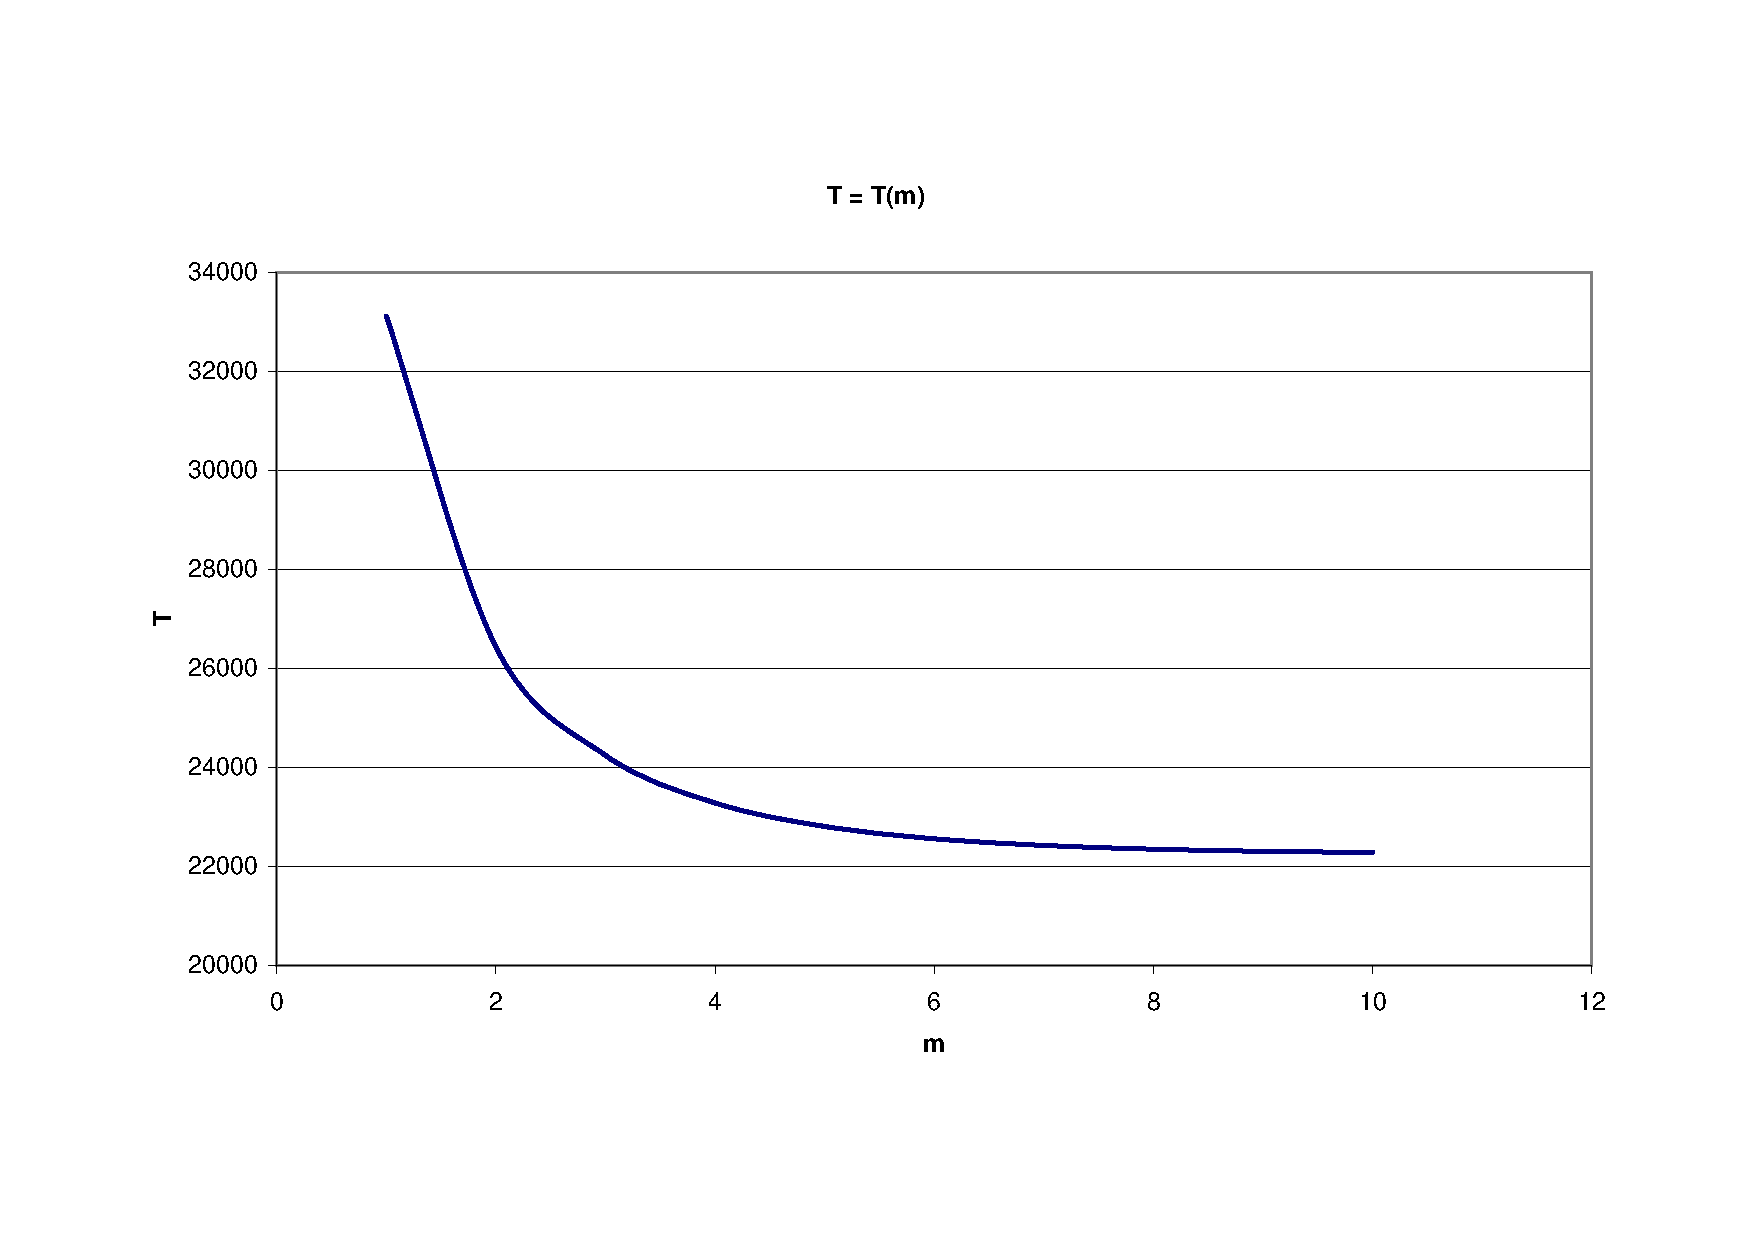
\includegraphics[width=\textwidth, trim=20mm 30mm 20mm 30mm, clip]{Simulation}
\caption{Zale�no�� czasu przetwarzania od liczby faz komunikacji}
\label{fig:Simulation}
\end{figure}

Czas przetwarzania w~systemie Parastation z procesorami o pr�dko�ciach $A_1$ i~$A_2$, przy za�o�eniu, �e w~chwili $t=0$ dane znajduj� si� ju� we wszystkich procesorach, jest opisany r�wnaniem:

$$T_{min} = V \; \frac{1}{\frac{4}{A_1} + \frac{4}{A_2}}$$

Dla przyj�tych danych czas ten wynosi $T_{min} \approx 22222$. Przedstawiony wykres pokazuje, �e wraz ze wzrostem ilo�ci faz komunikacji czas przetwarzania zbli�a si� asymptotycznie do tej granicy.

Diagramy Gantta odpowiadaj�ce rozwi�zaniom dla ilo�ci faz 1, 3 i~5 przedstawiaj� wykresy na rysunkach \ref{fig:SimulationGantt1}, \ref{fig:SimulationGantt3} i \ref{fig:SimulationGantt5}. Poszczeg�lne kana�y zosta�y pogrupowane wed�ug numer�w procesor�w, do kt�rych s� prowadz�, a obok wykres�w przedstawiaj�cych ich transmisj� w nich zachodz�ce umieszczono informacj� o �cie�ce, kt�r� pod��a�y dane. Liczby na samym wykresie informuj� o numerze fazy, w kt�rej dany pakiet zosta� przes�any.

\begin{figure}[p]
\centering
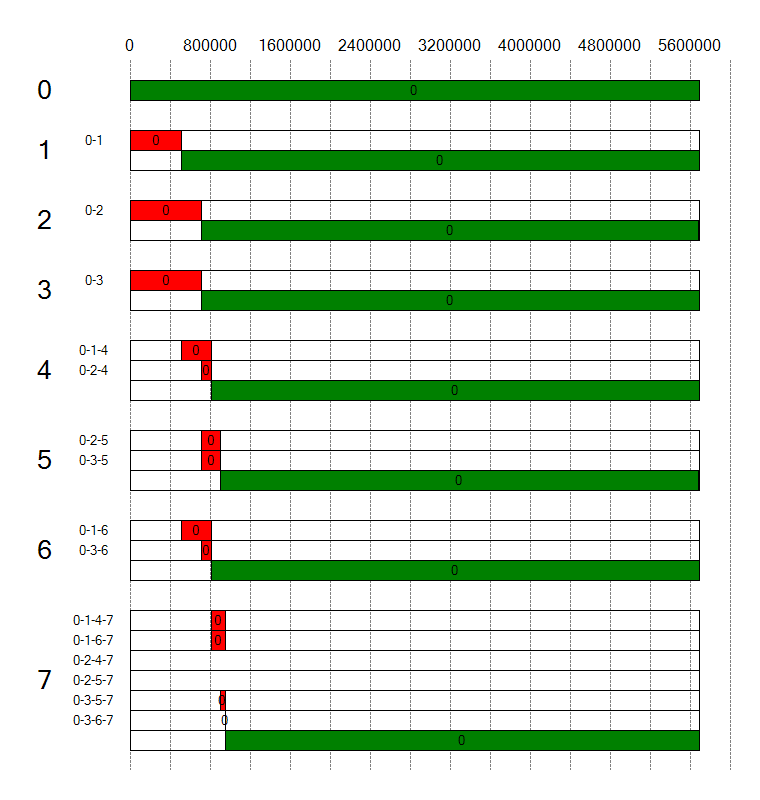
\includegraphics[width=\textwidth, trim=0 0 0 0, clip]{SimulationGantt1}
\caption{Diagram Gantta dla symulacji rozwi�zania z liczb� faz $m=1$}
\label{fig:SimulationGantt1}
\end{figure}

\begin{figure}[p]
\centering
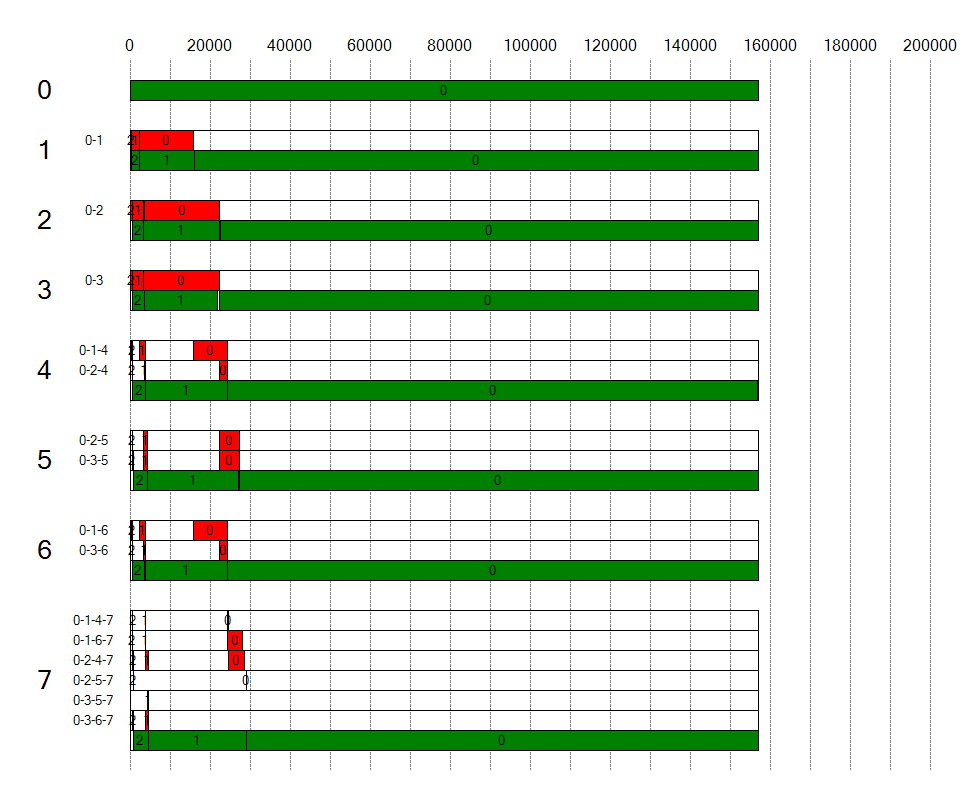
\includegraphics[width=\textwidth, trim=0 0 0 0, clip]{SimulationGantt3}
\caption{Diagram Gantta dla symulacji rozwi�zania z liczb� faz $m=3$}
\label{fig:SimulationGantt3}
\end{figure}

\begin{figure}[p]
\centering
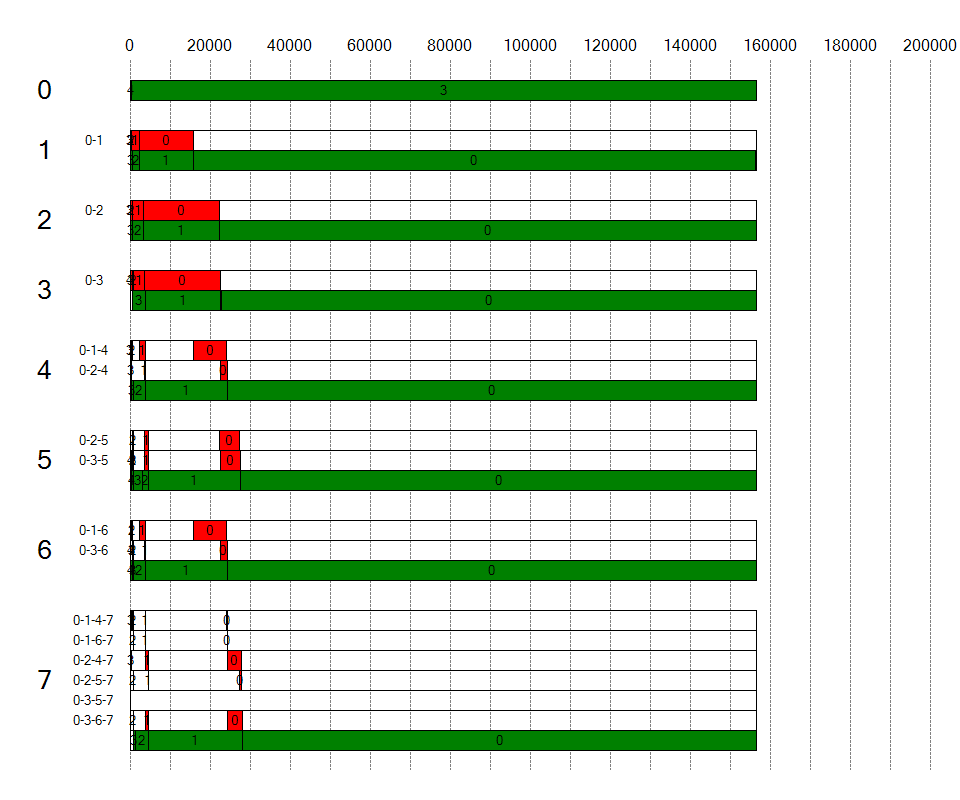
\includegraphics[width=\textwidth, trim=0 0 0 0, clip]{SimulationGantt5}
\caption{Diagram Gantta dla symulacji rozwi�zania z liczb� faz $m=5$}
\label{fig:SimulationGantt5}
\end{figure}

\section{Rozwi�zanie rzeczywiste}

\subsection{Struktura rozwi�zania}

W rozwi�zaniu problemy wykorzystano procesory przedstawione na rysunku \ref{fig:ProblemParastation}. Odpowiedni schemat wykonany w programie \emph{TransputerStudio} przedstawia rysunek \ref{fig:SolutionProcessors}.

\begin{figure}[h!]
\centering
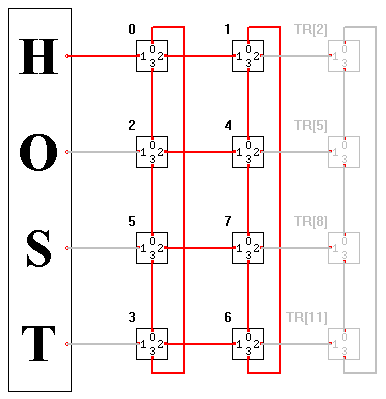
\includegraphics[width=8cm, trim=0 0 0 0, clip]{SolutionProcessors}
\caption{Procesory wykorzystywane podczas wykonywania pomiar�w}
\label{fig:SolutionProcessors}
\end{figure}

Ka�demu z procesor�w przypisano proces licz�cy (L) oraz odpowiedni� ilo�� proces�w odbieraj�cych (O) i wysy�aj�cych (W). W przypadku procesora 0 wyst�puje r�wnie� proces wej�cia/wyj�cia wymieniaj�cy dane z hostem oraz proces DEBUG, po�rednicz�cy przy zbieraniu danych o czasie oblicze�. Jego zastosowanie by�o konieczne ze wzgl�du na niewystarczaj�c� liczb� ��czy w procesie wej�cia/wyj�cia. Schemat po��cze� proces�w wykonany w programie \emph{TransputerStudio} przedstawia rysunek \ref{fig:SolutionProcessesGrouped}. Procesy zosta�y pogrupowane wed�ug numeru procesora, na kt�rym si� wykonuj� -- zgodnie z rysunkiem \ref{fig:ProblemFlat}.

Oznaczenia liczbowe w nazwach proces�w informuj� o parze procesor�w, pomi�dzy kt�rymi zachodzi komunikacja -- dla proces�w komunikacyjnych -- oraz o procesorze, na kt�rym wykonywane s� obliczenia -- dla proces�w licz�cych.

\begin{figure}[h!]
\centering
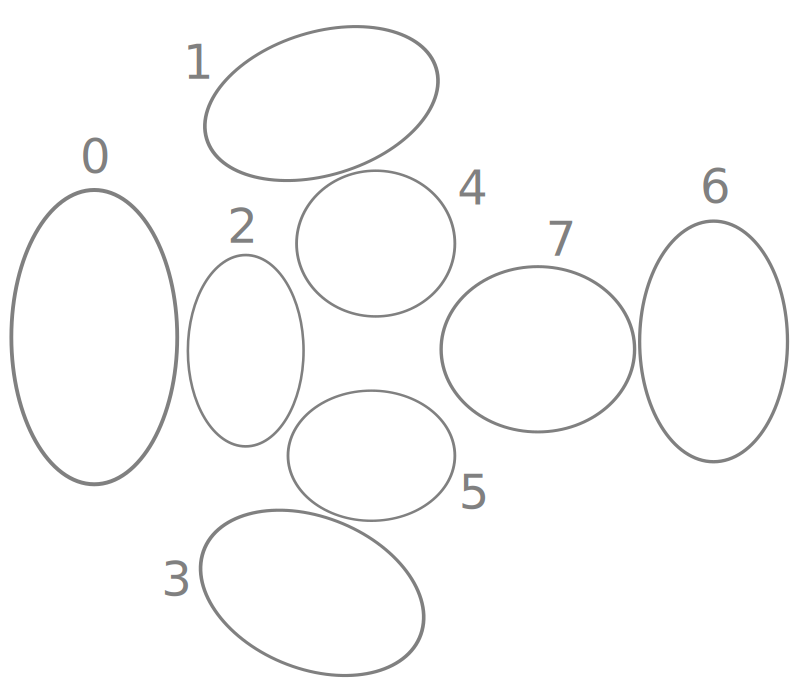
\includegraphics[width=\textwidth, trim=0 0 0 0, clip]{SolutionProcessesGrouped}
\caption{Procesy wykorzystywane podczas wykonywania pomiar�w}
\label{fig:SolutionProcesses}
\end{figure}

Dla ka�dego z przedstawionych typ�w proces�w wyst�puje tylko jeden og�lny kod programu. R�ne zachowanie proces�w uzyskuje si� poprzez przekazanie programom parametr�w konfiguracyjnych, okre�lajaj�cych: numer procesora �r�d�owego, numer procesora docelowego oraz ilo�� �r�de�/cel�w komunikacji.

Przy pomocy wymienionych wy�ej parametr�w mo�liwe jest zainicjowanie odpowiednich ��czy komunikacyjnych oraz pobranie rozmiar�w pakiet�w ze specjalnej tablicy $sizes$, generowanej na podstawie rozwi�zania opisanego wcze�niej problemu programowania liniowego.

\subsection{Pomiar czasu dzia�ania}

Do por�wnania z wynikami symulacji wybrano wariant z liczb� faz komunikacji $m=3$. Na podstawie zebranych danych sporz�dzono diagram Gantta przedstawiony na rysunku.

\begin{figure}[h!]
\centering
%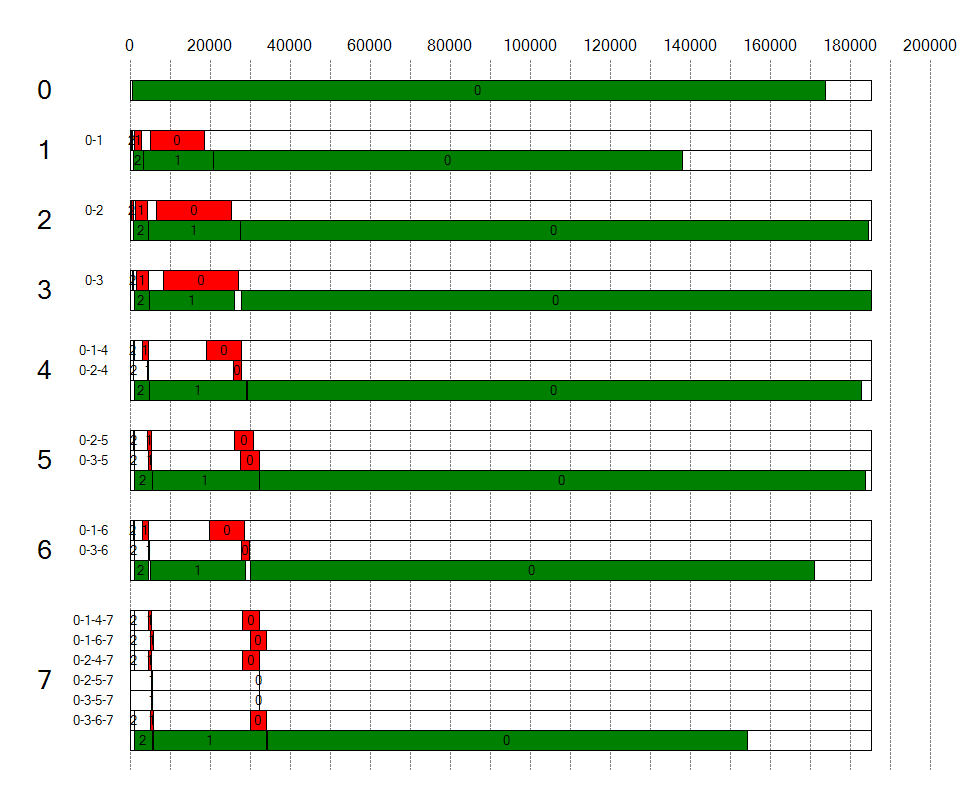
\includegraphics[width=\textwidth, trim=0 0 0 0, clip]{SolutionGantt3}
\caption{Diagram Gantta dla rozwi�zania rzeczywiste z liczb� faz $m=3$}
\label{fig:SolutionGantt3}
\end{figure}


\end{document}
